% ============================================================
\part{از مسئله فیزیکی تا جریان کاری}
% ============================================================

\chapter{از مسئله فیزیکی تا هامیلتونی}
\label{chap:models}

\section{جایگاه در نقشه}

بالای نمودار فصل~\ref{chap:map}: مسئله فیزیکی $\to$ مدل ریاضی $\to$ هامیلتونی $H$. قبل از انتخاب \lr{Trotter} یا \lr{VQE} باید معلوم شود $H$ چیست، از کجا آمده، و جمله‌هایش چه ساختاری دارند. بخش‌های~\ref{sec:phys-to-model}--\ref{sec:lc-quantize} همان زیربنا را می‌سازند؛ بخش~\ref{sec:ising} نمونه اسپینیِ پرکاربرد سند است.

\section{ایده شهودی}

فیزیک خام مستقیماً الگوریتم نمی‌شود. زنجیره درست این است: مسئله آزمایشگاهی $\to$ مدل ریاضیِ ایده‌آل‌شده که درجات آزادیِ مهم را نگه می‌دارد $\to$ هامیلتونی به‌عنوان مولد دینامیک و طیف $\to$ انتخاب پرسش (دینامیک یا پایه/طیف) $\to$ رهیافت و ابزار. شکل~\ref{fig:phys-to-H} همین اسکلت را نشان می‌دهد. بقیه این فصل همان زنجیره را از مکانیک کلاسیک تا کوانتشِ یک مدار \lr{LC} باز می‌کند؛ سپس خانواده‌های مدل رایج در شبیه‌سازی، و سرانجام \lr{Ising} به‌تفصیل می‌آید.

\begin{figure}[htbp]
	\centering
	\begin{latin}
		\setstretch{1}
		\resizebox{\ifdim\width>\textwidth\textwidth\else\width\fi}{!}{%
			% زنجیره: مسئله فیزیکی → مدل → درجات آزادی → هامیلتونی → پرسش
% سبک مشترک نمودارهای سند پایه‌ها (فقط داخل محیط latin فراخوانی شود)
\tikzset{
	qafbox/.style={
		draw=black!55,
		rounded corners=2pt,
		align=center,
		inner sep=3pt,
		thick,
		fill=white,
		font=\footnotesize\linespread{1}\selectfont,
		minimum height=0.95cm
	},
	qafwide/.style={
		qafbox,
		text width=2.55cm
	},
	qafnarr/.style={
		qafbox,
		text width=2.05cm
	},
	qaftitle/.style={
		font=\small\bfseries\linespread{1}\selectfont,
		align=center
	},
	qafarr/.style={
		-{Latex[length=2.2mm]},
		thick,
		draw=black!65
	},
	qafpanel/.style={
		draw,
		thick,
		rounded corners=4pt,
		inner xsep=8pt,
		inner ysep=8pt
	}
}

\begin{tikzpicture}[
	x=1cm,
	y=1cm,
	execute at begin picture={\hyphenpenalty=10000 \exhyphenpenalty=10000},
	box/.style={qafbox, text width=2.05cm, minimum height=1.15cm},
	note/.style={font=\scriptsize, text=black!55, align=center}
	]
	\node[box, fill=blue!14] (phys) at (0,0) {Physical\\problem};
	\node[box, fill=blue!10] (mod) at (2.9,0) {Idealized\\model};
	\node[box, fill=cyan!12] (dof) at (5.8,0) {Keep\\degrees of freedom};
	\node[box, fill=green!12] (H) at (8.7,0) {Hamiltonian\\$H(q,p)$ or $\hat H$};
	\node[box, fill=orange!14] (q) at (11.6,0) {Choose\\question};

	\draw[qafarr] (phys) -- (mod);
	\draw[qafarr] (mod) -- (dof);
	\draw[qafarr] (dof) -- (H);
	\draw[qafarr] (H) -- (q);

	\node[note, below=8pt of phys] {lab / material};
	\node[note, below=8pt of mod] {drop irrelevant\\detail};
	\node[note, below=8pt of dof] {spins, modes,\\orbitals,\ldots};
	\node[note, below=8pt of H] {generator of\\dynamics \& spectrum};
	\node[note, below=8pt of q] {dynamics vs\\ground state};
\end{tikzpicture}
%
		}
	\end{latin}
	\caption{از مسئله فیزیکی تا هامیلتونی و انتخاب پرسش. الگوریتم از اینجا به بعد شروع می‌شود، نه از خودِ آزمایشگاه.}
	\label{fig:phys-to-H}
\end{figure}

\section{از مسئله فیزیکی تا مدل ریاضی}
\label{sec:phys-to-model}

مدل، رونوشت وفادارِ جهان نیست؛ فشرده‌سازیِ آگاهانه است. آنچه نگه می‌دارید همان \emph{درجات آزادی} است که به سؤال پژوهشی‌تان جواب می‌دهد؛ بقیه را دور می‌ریزید یا در پارامترهای مؤثر جمع می‌کنید.

\paragraph{قاعده عملی.}
\begin{enumerate}
	\item سؤال را روشن کنید (چه مشاهده‌پذیری؟ در چه مقیاس زمانی/انرژی؟).
	\item درجات آزادیِ حداقلی را نام ببرید (اسپین سایت‌ها، اوربیتال‌ها، شار و بار مدار، \ldots).
	\item برهم‌کنش‌ها و قیدها را بنویسید.
	\item خروجی را به یک هامیلتونی (کلاسیک یا کوانتومی) برسانید.
\end{enumerate}

\paragraph{چند مسئله واقعی و مدل نماینده.}
جدول~\ref{tab:phys-examples} نشان می‌دهد که \emph{همان ماده} بسته به پرسش، مدل متفاوتی می‌گیرد.

\begin{table}[htbp]
	\centering
	\footnotesize
	\setstretch{1.12}
	\caption{نمونه مسئله فیزیکی، مدل ریاضی، درجات آزادی، و پرسش نوعی.}
	\label{tab:phys-examples}
	\begin{tabularx}{\textwidth}{@{}
			>{\raggedright\arraybackslash}p{2.8cm}
			>{\raggedright\arraybackslash}p{2.6cm}
			>{\raggedright\arraybackslash}p{2.8cm}
			>{\raggedright\arraybackslash}X
			@{}}
		\toprule
		\rowcolor{gray!14}
		\textbf{مسئله فیزیکی} & \textbf{مدل نماینده} & \textbf{درجات آزادی} & \textbf{پرسش نوعی} \\
		\midrule
		آهن‌ربا / اسپین شیشه
		& \lr{Ising} / \lr{Heisenberg}
		& اسپین روی شبکه
		& پیکربندی پایه؛ گاف؛ دینامیک پس از quench
		\\
		\rowcolor{gray!8}
		الکترون در اکسید همبسته
		& فرمی-هابارد
		& الکترون روی سایت با اسپین
		& عایق مات در برابر فلز؛ ترابرد؛ quench
		\\
		مولکول کوچک / کاتالیز
		& ساختار الکترونی (\lr{ab initio})
		& اوربیتال‌های فعال
		& انرژی پایه؛ طیف ارتعاشی--الکترونی
		\\
		\rowcolor{gray!8}
		مدار ابررسانا / کاواک
		& نوسانگر / مدار \lr{LC} (بعداً غیرخطی)
		& شار و بار (مد بوزونی)
		& بسامد؛ واپاشی؛ جفت‌شدگی به کیوبیت
		\\
		یون در تله / اتم در شبکه نوری
		& نوسانگر مکانیکی یا بوز-هابارد
		& مدهای حرکت یا اشغال سایت
		& سرمایش؛ تونل‌زنی؛ شبیه‌سازی آنالوگ
		\\
		\bottomrule
	\end{tabularx}
\end{table}

نکته کلیدی: «پاسخی که انتظار دارید» مدل را انتخاب می‌کند. اگر فقط انرژی پایه یک آرایش اسپینی می‌خواهید، \lr{Ising} کلاسیک کافی است. اگر دینامیک همدوس و درهم‌تنیدگی مهم است، باید مدل کوانتومی (مثلاً \lr{TFIM} یا هابارد) بگیرید. اگر سخت‌افزار خود یک کاواک است، زبان طبیعی همان نوسانگر هماهنگ کوانتومی است.

\section{هامیلتونی کلاسیک: از کجا می‌آید و چرا مهم است؟}
\label{sec:classical-H}

در مکانیک تحلیلی، وضعیت سامانه با مختصات تعمیم‌یافته $q$ و تکانه‌های مزدوج $p$ توصیف می‌شود. لاگرانژی $L(q,\dot q,t)$ را از انرژی جنبشی و پتانسیل می‌سازید؛ هامیلتونی تبدیل لژاندرِ آن است:
\begin{equation}
	\label{eq:classical-H}
	H(q,p,t) = \sum_i p_i\dot q_i - L,
	\qquad
	p_i=\frac{\partial L}{\partial\dot q_i}.
\end{equation}
برای سامانه‌های پایستارِ متداول، $H$ همان انرژی کل برحسب $(q,p)$ است. معادلات حرکت هامیلتون:
\begin{equation}
	\dot q_i = \frac{\partial H}{\partial p_i},
	\qquad
	\dot p_i = -\frac{\partial H}{\partial q_i}.
\end{equation}
پس $H$ دو نقش هم‌زمان دارد: (۱) \emph{انرژی} روی فضای فاز، و (۲) \emph{مولد} تحول زمانیِ کلاسیک.

\paragraph{کمینه‌سازی چه معنایی دارد؟}
\begin{itemize}
	\item در تعادل استاتیک، پیکربندی‌های پایدار اغلب نقاط بحرانیِ انرژی پتانسیل‌اند (کمینه موضعی).
	\item در بهینه‌سازی ترکیبیاتیِ نگاشته‌شده به \lr{Ising}، «جواب» همان آرگ‌مینِ یک تابع انرژی روی پیکربندی‌های گسسته است --- همان نقش $H_{\mathrm{Ising}}$ در بخش~\ref{sec:ising}.
	\item در دینامیک، مسیر واقعی لزوماً «کمینه کردن $H$ در هر لحظه» نیست؛ $H$ در سامانه‌های پایستار ثابت می‌ماند و مسیر از معادلات هامیلتون می‌آید. کمینه‌سازیِ انرژی وقتی معنا دارد که دنبال حالت تعادل / پایه باشید، نه وقتی فیلم حرکت می‌خواهید.
\end{itemize}

\paragraph{مثال کوچک کلاسیک: نوسانگر یک‌بعدی.}
\begin{equation}
	H(x,p)=\frac{p^2}{2m}+\frac12 m\omega^2 x^2.
\end{equation}
کمینه انرژی در $(x,p)=(0,0)$ است؛ حرکت حول همان نقطه نوسان می‌کند. همین مدل بعد از کوانتش، آجرِ بسیاری از نظریه‌های میدان، اپتیک کوانتومی، و مدارهای ابررساناست.

\section{هامیلتونی کوانتومی}
\label{sec:quantum-H}

کوانتش کانونی می‌گوید: زوج‌های $(q,p)$ را به عملگرهای $(\hat q,\hat p)$ با
\begin{equation}
	\label{eq:ccr}
	[\hat q,\hat p]=i\hbar
\end{equation}
ارتقاء دهید و $H(q,p)$ را به عملگر $\hat H=H(\hat q,\hat p)$ تبدیل کنید (با ترتیب عملگرهای مناسب). دینامیک دیگر معادله هامیلتون نیست؛ معادله شرودینگر است:
\begin{equation}
	i\hbar\,\partial_t\lvert\psi\rangle = \hat H\lvert\psi\rangle,
\end{equation}
و طیف $\hat H\lvert E_n\rangle=E_n\lvert E_n\rangle$ انرژی‌های مجاز را می‌دهد. در بقیه این سند، نماد $H$ معمولاً همین عملگر کوانتومی است.

\paragraph{چرا در شبیه‌سازی کوانتومی مرکز صحنه است؟}
چون تقریباً همه پرسش‌های این سند تابعی از یک $H$اند: $e^{-iHt}$، ویژه‌مقدارها، $\langle O\rangle$ روی پایه، مسیر $H(s)$، یا $f(H)$. بدون تثبیت $H$ و درجات آزادی‌اش، انتخاب \lr{Trotter} یا \lr{VQE} زودرس است.

\section{نوسانگر هماهنگ و عملگرهای خلق و فنا}
\label{sec:harmonic}

نوسانگر هماهنگ کوانتومی هم مدل فیزیکی است و هم زبان مشترک برای مدهای بوزونی (کاواک، فونون، مدار \lr{LC}).

\paragraph{هامیلتونی و طیف.}
با $\hbar=1$ برای سادگی سند،
\begin{equation}
	\label{eq:sho}
	H = \frac{p^2}{2m}+\frac12 m\omega^2 x^2
	= \omega\Bigl(a^\dagger a+\tfrac12\Bigr),
\end{equation}
که عملگرهای بی‌بعد
\begin{equation}
	a=\sqrt{\frac{m\omega}{2}}\Bigl(x+\frac{i}{m\omega}p\Bigr),
	\qquad
	a^\dagger=\sqrt{\frac{m\omega}{2}}\Bigl(x-\frac{i}{m\omega}p\Bigr)
\end{equation}
در جبر بوزونی صدق می‌کنند:
\begin{equation}
	[a,a^\dagger]=1,
	\qquad
	[a,a]=[a^\dagger,a^\dagger]=0.
\end{equation}
ویژه‌حالت‌های عددی $\lvert n\rangle$ با $a^\dagger a\lvert n\rangle=n\lvert n\rangle$ و انرژی $E_n=\omega(n+\tfrac12)$ همان نردبان شکل~\ref{fig:harmonic-osc}اند. $a$ یک کوانتوم کم می‌کند (فنا)، $a^\dagger$ یکی اضافه می‌کند (خلق).

\begin{figure}[htbp]
	\centering
	\begin{latin}
		\setstretch{1}
		\resizebox{0.55\textwidth}{!}{%
			% نوسانگر هماهنگ: پتانسیل و ترازها (طرحواره)
% سبک مشترک نمودارهای سند پایه‌ها (فقط داخل محیط latin فراخوانی شود)
\tikzset{
	qafbox/.style={
		draw=black!55,
		rounded corners=2pt,
		align=center,
		inner sep=3pt,
		thick,
		fill=white,
		font=\footnotesize\linespread{1}\selectfont,
		minimum height=0.95cm
	},
	qafwide/.style={
		qafbox,
		text width=2.55cm
	},
	qafnarr/.style={
		qafbox,
		text width=2.05cm
	},
	qaftitle/.style={
		font=\small\bfseries\linespread{1}\selectfont,
		align=center
	},
	qafarr/.style={
		-{Latex[length=2.2mm]},
		thick,
		draw=black!65
	},
	qafpanel/.style={
		draw,
		thick,
		rounded corners=4pt,
		inner xsep=8pt,
		inner ysep=8pt
	}
}

\begin{tikzpicture}[
	x=1.1cm,
	y=0.9cm,
	note/.style={font=\scriptsize, text=black!55}
	]
	\draw[->, thick] (-2.2,0) -- (2.4,0) node[right] {$x$};
	\draw[->, thick] (0,-0.3) -- (0,3.2) node[above] {$V(x)$};
	\draw[thick, blue!70!black, domain=-1.9:1.9, samples=60]
		plot (\x, {0.55*\x*\x});
	\draw[thick, black!50] (-1.55,1.3) -- (1.55,1.3);
	\draw[thick, black!50] (-1.85,1.95) -- (1.85,1.95);
	\draw[thick, black!50] (-2.05,2.55) -- (2.05,2.55);
	\node[note, right] at (1.6,1.3) {$E_0$};
	\node[note, right] at (1.9,1.95) {$E_1$};
	\node[note, right] at (2.1,2.55) {$E_2$};
	\node[note] at (0,-0.7) {$V=\tfrac12 m\omega^2 x^2$};
\end{tikzpicture}
%
		}
	\end{latin}
	\caption{طرحواره پتانسیل هماهنگ و ترازهای هم‌فاصله $E_n$. غیرخطی‌سازی بعدی فاصله ترازها را به هم می‌زند و راه ساخت کیوبیت از مدار را باز می‌کند.}
	\label{fig:harmonic-osc}
\end{figure}

\paragraph{نوسانگر واداشته.}
اگر نیروی خارجی یا جفت‌شدگی به میدانِ رانش باشد،
\begin{equation}
	H(t)=\omega\Bigl(a^\dagger a+\tfrac12\Bigr)+\bigl(\varepsilon(t)\,a^\dagger+\varepsilon^*(t)\,a\bigr),
\end{equation}
مد را جابه‌جا یا همدوس می‌رانید. در اپتیک کوانتومی و کنترل کاواک، همین جمله‌های خطیِ رانش ابزار استانداردند.

\paragraph{نقش در نظریه‌های مرتبط.}
\begin{itemize}
	\item هر مدِ هارمونیکِ مستقل $=$ یک نسخه از~\eqref{eq:sho}.
	\item میدان آزاد در کاواک یا موجبر: مجموعه مدها با $a_k,a_k^\dagger$.
	\item جفت‌شدگی به اتم / کیوبیت: مدل‌های جینز--کامینگز و خویشاوندانش ($g(a\sigma^++a^\dagger\sigma^-)$).
	\item در مدارهای ابررسانا: ابتدا \lr{LC} هماهنگ است؛ برای داشتن دو ترازِ نشانی‌پذیر باید غیرخطی (پیوند جوزفسون) اضافه شود --- جای توسعه در فصل سخت‌افزار/کیوبیت.
\end{itemize}

\paragraph{نوشتن $H$ سیستم‌های بس‌مدی با خلق و فنا.}
الگوی کلی برای بوزون‌ها:
\begin{equation}
	H
	=
	\sum_k \omega_k a_k^\dagger a_k
	+
	\sum_{k\ell} g_{k\ell}\,a_k^\dagger a_\ell
	+
	\cdots
\end{equation}
و برای فرمیون‌ها با $c,c^\dagger$ و $\{c_i,c_j^\dagger\}=\delta_{ij}$ (هابارد و شیمی همین زبان را دارند؛ نگاشت به کیوبیت جداگانه است).

\section{مثال کاری: مدار \lr{LC} از کلاسیک تا کوانتوم}
\label{sec:lc-quantize}

یک مدار متشکل از القاگر $L$ و خازن $C$ ساده‌ترین سخت‌افزارِ نوسانگر الکتریکی است و پل مستقیم به مدارهای کوانتومی ابررساناست. شکل~\ref{fig:lc-circuit} متغیرهای کانونی را نشان می‌دهد.

\begin{figure}[htbp]
	\centering
	\begin{latin}
		\setstretch{1}
		\resizebox{0.85\textwidth}{!}{%
			% مدار LC کلاسیک و زوج کانونی (Φ, Q)
% سبک مشترک نمودارهای سند پایه‌ها (فقط داخل محیط latin فراخوانی شود)
\tikzset{
	qafbox/.style={
		draw=black!55,
		rounded corners=2pt,
		align=center,
		inner sep=3pt,
		thick,
		fill=white,
		font=\footnotesize\linespread{1}\selectfont,
		minimum height=0.95cm
	},
	qafwide/.style={
		qafbox,
		text width=2.55cm
	},
	qafnarr/.style={
		qafbox,
		text width=2.05cm
	},
	qaftitle/.style={
		font=\small\bfseries\linespread{1}\selectfont,
		align=center
	},
	qafarr/.style={
		-{Latex[length=2.2mm]},
		thick,
		draw=black!65
	},
	qafpanel/.style={
		draw,
		thick,
		rounded corners=4pt,
		inner xsep=8pt,
		inner ysep=8pt
	}
}

\begin{tikzpicture}[
	x=1cm,
	y=1cm,
	note/.style={font=\scriptsize, text=black!60, align=center}
	]
	% inductor box
	\draw[thick] (0,0.8) -- (0,1.4);
	\draw[thick] (0,1.4) -- (0.15,1.55) -- (0.35,1.25) -- (0.55,1.55) -- (0.75,1.25)
		-- (0.95,1.55) -- (1.15,1.25) -- (1.35,1.55) -- (1.5,1.4) -- (1.5,0.8);
	\node[note] at (0.75,2.05) {$L$};
	% capacitor
	\draw[thick] (0,0.8) -- (0,0.2) -- (0.55,0.2);
	\draw[thick] (0.55,0.05) -- (0.55,0.35);
	\draw[thick] (0.75,0.05) -- (0.75,0.35);
	\draw[thick] (0.75,0.2) -- (1.5,0.2) -- (1.5,0.8);
	\node[note] at (0.65,-0.25) {$C$};

	\node[note, text width=4.2cm, align=left] at (4.6,1.0) {%
		Canonical pair:\\[2pt]
		flux $\Phi$, charge $Q$\\[2pt]
		$H=\dfrac{Q^2}{2C}+\dfrac{\Phi^2}{2L}$\\[2pt]
		quantize: $[\hat\Phi,\hat Q]=i\hbar$};
\end{tikzpicture}
%
		}
	\end{latin}
	\caption{مدار \lr{LC}: انرژی مغناطیسی در $L$ و الکتریکی در $C$. زوج کانونی معمول شار گره $\Phi$ و بار گره $Q$ است.}
	\label{fig:lc-circuit}
\end{figure}

\paragraph{گام ۱ --- انرژی کلاسیک.}
شار $\Phi$ از القاگر و بار $Q$ روی خازن را مختصات کانونی بگیرید. انرژی کل
\begin{equation}
	\label{eq:lc-classical}
	H(\Phi,Q)
	=
	\frac{Q^2}{2C}
	+
	\frac{\Phi^2}{2L}
\end{equation}
است (الکتریکی $+$ مغناطیسی). این دقیقاً همان شکل نوسانگر است با «جرم» و «فنر» بازتعریف‌شده؛ بسامد زاویه‌ای
\begin{equation}
	\omega = \frac{1}{\sqrt{LC}}.
\end{equation}

\paragraph{گام ۲ --- کوانتش.}
عملگرهای $\hat\Phi,\hat Q$ را با
\begin{equation}
	[\hat\Phi,\hat Q]=i\hbar
\end{equation}
معرفی کنید و~\eqref{eq:lc-classical} را عملگری بخوانید. با تعریف
\begin{equation}
	a
	=
	\frac{1}{\sqrt{2\hbar Z}}
	\bigl(\hat\Phi + i Z\hat Q\bigr),
	\qquad
	Z=\sqrt{\frac{L}{C}},
\end{equation}
دوباره به
\begin{equation}
	\hat H = \hbar\omega\Bigl(a^\dagger a+\tfrac12\Bigr)
\end{equation}
می‌رسید --- همان~\eqref{eq:sho}. طیف هم‌فاصله است؛ دو تراز اول به‌تنهایی یک کیوبیتِ خوب نمی‌سازند چون $E_1-E_0=E_2-E_1$.

\paragraph{گام ۳ --- پیام برای ادامه سند.}
\begin{itemize}
	\item اگر هدف شبیه‌سازیِ یک مد هارمونیک یا جفت‌شدگی خطی به آن است، همین $H$ کافی است.
	\item اگر هدف \emph{کیوبیت} از مدار است، باید پتانسیل را غیرهارمونیک کرد (پیوند جوزفسون: جمله $-\,E_J\cos(\hat\Phi/\phi_0)$). آن‌گاه فاصله ترازها یکنواخت نیست و می‌توان دو تراز را آدرس‌دهی کرد. جزئیات مهندسی کیوبیت ابررسانا جای توسعه فصل~\ref{chap:hardware} است؛ اینجا فقط زنجیره منطقی را قفل می‌کنیم: فیزیک مدار $\to$ $H$ کلاسیک $\to$ کوانتش با جابجاگر $\to$ (در صورت نیاز) غیرخطی‌سازی.
\end{itemize}

\section{خانواده‌های مدل در شبیه‌سازی کوانتومی}

پس از تثبیت زبان $H$، چهار خانواده برای جهت‌یابی پژوهش کافی‌اند. آنچه از مدلی به مدل دیگر عوض می‌شود کدگذاری درجات آزادی و نوع جمله‌هاست، نه اسکلت الگوریتم.

\paragraph{اسپین: \lr{Ising} و \lr{Heisenberg}.}
ساده‌ترین ورود. درجات آزادی اسپین روی شبکه؛ $H$ جمع جمله‌های دو جسمی مثل $Z_i Z_j$ یا $\vec{S}_i\cdot\vec{S}_j$. شهود: مغناطیس، شیشه اسپینی، و بسیاری مسائل بهینه‌سازی که به \lr{Ising} نگاشته می‌شوند. شرح پایه در بخش~\ref{sec:ising}.

\paragraph{هابارد (فرمی و بوز).}
مدل استاندارد همبستگی قوی: ذرات روی شبکه می‌پرند ($t$) و اگر روی یک سایت باشند انرژی $U$ می‌پردازند. فرمی-هابارد الکترون‌های همبسته است؛ بوز-هابارد اتم‌های سرد در شبکه نوری. پرسش‌های نوعی: عایق مات، ابرشاره، ترابرد، دینامیک پس از تغییر ناگهانی هامیلتونی. زبان فرمیونی همان $c,c^\dagger$ است.

\paragraph{ساختار الکترونی مولکولی.}
الکترون‌ها در میدان هسته‌ها. پس از انتخاب پایه و اغلب یک فضای فعال،\footnote{\lr{active space}.} $H$ به شکل فرمیونی یا پائولی درمی‌آید~\cite{McArdle2020,Bauer2020}. شیمی کوانتومی از همین‌جا به \lr{VQE} و به شبیه‌سازی تحمل‌پذیر در برابر خطا وصل می‌شود.

\paragraph{میدان روی شبکه و نظریه پیمانه‌ای شبکه‌ای.}
میدان کوانتومی پیوسته را روی شبکه می‌نشانند تا درجات آزادی متناهی شود. نظریه‌های پیمانه‌ای قیدهای موضعی (قانون گاوس) دارند؛ همین قیدها کدگذاری را سخت‌تر از هابارد می‌کنند. مدهای پیمانه‌ای اغلب خویشاوند نوسانگر / روتورند.

\section{مدل \lr{Ising}: از فیزیک تا کیوبیت}
\label{sec:ising}

این بخش برای کسی نوشته شده که هنوز با نظریه \lr{Ising} کار نکرده است. هدف، نه تاریخچه کامل فیزیک آماری، بلکه همان زبانی است که در بقیه این سند (آدیاباتیک، \lr{QAOA}، بهینه‌سازی) به کار می‌رود.

\subsection{ایده فیزیکی}

روی هر سایت شبکه یک اسپین دارید که دو حالت دارد: بالا یا پایین. در مغناطیس، این‌ها جهت ممان مغناطیسی موضعی‌اند؛ در محاسبات کوانتومی همان دو حالت را با یک کیوبیت نشان می‌دهیم:
\begin{equation}
	\lvert\uparrow\rangle \equiv \lvert0\rangle,
	\qquad
	\lvert\downarrow\rangle \equiv \lvert1\rangle.
\end{equation}
اسپین‌های همسایه می‌توانند بخواهند هم‌جهت بمانند (فرومغناطیس) یا مخالف هم بایستند (پادفرومغناطیس). میدان خارجی هم می‌تواند هر اسپین را به یک سمت هل بدهد. انرژی کل سامانه جمع همین ترجیح‌های موضعی است؛ \emph{پیکربندی پایه} همان آرایشی است که انرژی را کمینه می‌کند. شکل~\ref{fig:ising-lattice} یک تکه کوچک شبکه را نشان می‌دهد.

\begin{figure}[htbp]
	\centering
	\begin{latin}
		\setstretch{1}
		\resizebox{0.95\textwidth}{!}{%
			% شبکهٔ Ising: اسپین‌ها، جفت‌شدگی ZZ، میدان موضعی
% سبک مشترک نمودارهای سند پایه‌ها (فقط داخل محیط latin فراخوانی شود)
\tikzset{
	qafbox/.style={
		draw=black!55,
		rounded corners=2pt,
		align=center,
		inner sep=3pt,
		thick,
		fill=white,
		font=\footnotesize\linespread{1}\selectfont,
		minimum height=0.95cm
	},
	qafwide/.style={
		qafbox,
		text width=2.55cm
	},
	qafnarr/.style={
		qafbox,
		text width=2.05cm
	},
	qaftitle/.style={
		font=\small\bfseries\linespread{1}\selectfont,
		align=center
	},
	qafarr/.style={
		-{Latex[length=2.2mm]},
		thick,
		draw=black!65
	},
	qafpanel/.style={
		draw,
		thick,
		rounded corners=4pt,
		inner xsep=8pt,
		inner ysep=8pt
	}
}

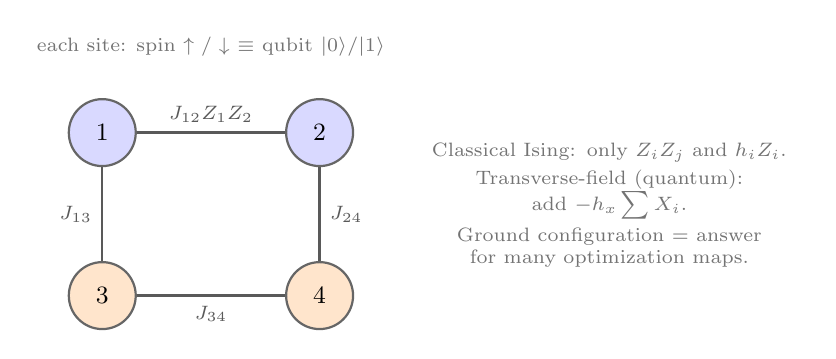
\begin{tikzpicture}[
	x=1.15cm,
	y=1.15cm,
	execute at begin picture={\hyphenpenalty=10000 \exhyphenpenalty=10000},
	spin/.style={circle, draw=black!60, thick, minimum size=0.85cm, inner sep=0pt, font=\small\bfseries},
	note/.style={font=\scriptsize, text=black!55, align=center}
	]
	\node[spin, fill=blue!15] (s1) at (0,1.2) {$1$};
	\node[spin, fill=blue!15] (s2) at (2.4,1.2) {$2$};
	\node[spin, fill=orange!20] (s3) at (0,-0.6) {$3$};
	\node[spin, fill=orange!20] (s4) at (2.4,-0.6) {$4$};

	\draw[thick, black!65] (s1) -- (s2) node[midway, above, font=\scriptsize] {$J_{12}Z_1Z_2$};
	\draw[thick, black!65] (s1) -- (s3) node[midway, left, font=\scriptsize] {$J_{13}$};
	\draw[thick, black!65] (s2) -- (s4) node[midway, right, font=\scriptsize] {$J_{24}$};
	\draw[thick, black!65] (s3) -- (s4) node[midway, below, font=\scriptsize] {$J_{34}$};

	\node[note] at (1.2,2.15) {each site: spin $\uparrow/\downarrow$ $\equiv$ qubit $|0\rangle/|1\rangle$};
	\node[note, text width=4.8cm] at (5.6,0.4) {%
		Classical Ising: only $Z_iZ_j$ and $h_i Z_i$.\\[2pt]
		Transverse-field (quantum): add $-h_x\sum X_i$.\\[2pt]
		Ground configuration $=$ answer for many optimization maps.};
\end{tikzpicture}
%
		}
	\end{latin}
	\caption{شبکه \lr{Ising}: هر رأس یک اسپین/کیوبیت، هر یال یک جفت‌شدگی $J_{ij}Z_iZ_j$، و در صورت نیاز میدان موضعی $h_i Z_i$.}
	\label{fig:ising-lattice}
\end{figure}

\subsection{هامیلتونی کلاسیک}

شکل استاندارد روی $n$ سایت:
\begin{equation}
	\label{eq:ising-classical}
	H_{\mathrm{Ising}}
	=
	\sum_{i<j} J_{ij}\, Z_i Z_j
	+
	\sum_{i} h_i\, Z_i.
\end{equation}
اینجا $Z_i$ همان ماتریس پائولی روی سایت $i$ است؛ روی پایه محاسباتی قطری است:
\begin{equation}
	Z\lvert0\rangle=+\lvert0\rangle,
	\qquad
	Z\lvert1\rangle=-\lvert1\rangle.
\end{equation}
پس روی هر رشته بیتی $z\in\{0,1\}^n$، $H_{\mathrm{Ising}}$ فقط یک عدد می‌دهد --- انرژی کلاسیک آن پیکربندی. به همین دلیل به آن \emph{\lr{Ising} کلاسیک} می‌گویند: ویژه‌حالت‌های انرژی همان پایه‌های محاسباتی‌اند و نیازی به برهم‌نهی نیست.

\paragraph{معنی علامت‌ها.}
برای یک جفت، جمله $J\,Z_i Z_j$ را نگاه کنید:
\begin{itemize}
	\item اگر هر دو $\lvert0\rangle$ یا هر دو $\lvert1\rangle$ باشند، $Z_iZ_j=+1$ و سهم انرژی $J$ است.
	\item اگر مخالف باشند، $Z_iZ_j=-1$ و سهم $-J$ است.
\end{itemize}
بنابراین:
\begin{itemize}
	\item $J<0$ (یا در قرارداد دیگر $J>0$ با علامت کلیِ منفی جلوی مجموع): هم‌جهتی انرژی را پایین می‌آورد --- \emph{فرومغناطیس}.
	\item علامت مخالف: مخالف‌بودن مطلوب است --- \emph{پادفرومغناطیس}.
\end{itemize}
در این سند اغلب می‌نویسیم $-J Z_i Z_j$ با $J>0$ تا فرومغناطیس صریح باشد (مثل مثال آدیاباتیک). میدان $h_i$ یک سمت را ترجیح می‌دهد؛ مثلاً $h_i>0$ در قرارداد $-h_i Z_i$ حالت $\lvert0\rangle$ را پایین می‌آورد.

\paragraph{پارامترها، یک‌جا.}
\begin{itemize}
	\item $n$: تعداد اسپین / کیوبیت.
	\item $J_{ij}$: قدرت و نوع جفت‌شدگی روی یال $(i,j)$.
	\item $h_i$: میدان طولی موضعی.
	\item پیکربندی پایه: رشته بیتی با کمینه انرژی؛ همان «جواب» بسیاری از نگاشت‌های بهینه‌سازی.
\end{itemize}

\subsection{مثال کامل: دو اسپین فرومغناطیس}

کوچک‌ترین شبکه غیربدیهی:
\begin{equation}
	\label{eq:ising-two}
	H = -J\, Z_1 Z_2 - h_z\,(Z_1+Z_2),
	\qquad
	J>0,\ h_z>0.
\end{equation}
روی چهار پایه محاسباتی انرژی‌ها صریح‌اند (همان جدول مثال آدیاباتیک):
\begin{equation}
	\begin{aligned}
		E(\lvert00\rangle) &= -J-2h_z,\\
		E(\lvert11\rangle) &= -J+2h_z,\\
		E(\lvert01\rangle) &= E(\lvert10\rangle) = +J.
	\end{aligned}
\end{equation}
پس برای $J,h_z>0$ حالت پایه یکتا $\lvert00\rangle$ است. اگر $h_z=0$، پایه‌های $\lvert00\rangle$ و $\lvert11\rangle$ تبهگن می‌شوند --- هر دو «هم‌جهت»اند و فرومغناطیس هر دو را یکسان دوست دارد. میدان طولی کوچک این تبهگنی را می‌شکند.

این همان $H_P$ در بخش~\ref{sec:adi-ising-example} و نزدیک به $H_C$ در بخش~\ref{sec:qaoa-example} است. تفاوت فصل‌ها در \emph{چگونه} به پایه می‌رسند است، نه در تعریف خودِ مدل.

\subsection{\lr{Ising} کوانتومی و میدان عرضی}

اگر فقط جمله‌های $Z$ داشته باشید، هامیلتونی با پایه محاسباتی جابه‌جا می‌شود و دینامیک کوانتومیِ غیربدیهی نمی‌سازد. با افزودن میدان \emph{عرضی}،
\begin{equation}
	\label{eq:tfim}
	H_{\mathrm{TFIM}}
	=
	-J\sum_{\langle ij\rangle} Z_i Z_j
	-
	h_x\sum_i X_i,
\end{equation}
جمله‌های $X$ پیکربندی‌های محاسباتی را مخلوط می‌کنند. این \emph{مدل \lr{Ising} در میدان عرضی}\footnote{\lr{transverse-field Ising model} (\lr{TFIM}).} است: یک مدل کوانتومیِ واقعی با درهم‌تنیدگی، گذار فاز کوانتومی، و دینامیک غیربدیهی.

در محاسبه آدیاباتیک، اغلب از حدِ فقط‌عرضی ($H_B=-h_x\sum X_i$) به‌سمت حدِ کلاسیک ($H_P$ فقط $Z$) حرکت می‌کنید؛ یعنی خودِ الگوریتم یک مسیر داخل خانواده~\eqref{eq:tfim} است.

\subsection{چرا در الگوریتم‌های کوانتومی این‌قدر دیده می‌شود؟}

\begin{enumerate}
	\item \textbf{کدگذاری طبیعی روی کیوبیت.} هر اسپین $=$ یک کیوبیت؛ جمله‌ها پائولی‌اند؛ برای مدار دیجیتال یا سخت‌افزار آنالوگ اسپینی آماده است.
	\item \textbf{نگاشت بهینه‌سازی.} بسیاری از مسائل ترکیبیاتی (\lr{MaxCut}، پوشش، تخصیص، \ldots) را می‌توان به یافتن پایه یک $H_{\mathrm{Ising}}$ ترجمه کرد؛ پس حل \lr{Ising} $=$ حل آن مسئله.
	\item \textbf{آزمونگاه روش‌ها.} کوچک است، قابل شمارش است، و در عین حال با زیاد شدن $n$ یا پیچیدگی $J_{ij}$ سخت می‌شود --- مناسب مثال‌های این سند و بنچمارک الگوریتم‌ها.
\end{enumerate}

\subsection{تمایزهای مهم}

\begin{itemize}
	\item \textbf{\lr{Ising} در برابر \lr{Heisenberg}.} در \lr{Heisenberg} جمله کامل $\vec{S}_i\cdot\vec{S}_j=X_iX_j+Y_iY_j+Z_iZ_j$ است؛ هر سه راستا در جفت‌شدگی شرکت دارند. \lr{Ising} فقط کانال $Z$ (به‌علاوه میدان‌های خارجی) را نگه می‌دارد.
	\item \textbf{مدل فیزیکی در برابر هزینه بهینه‌سازی.} گاهی $H_{\mathrm{Ising}}$ توصیف یک آهن‌ربا است؛ گاهی فقط تابع هزینه‌ای است که روی کیوبیت نوشته‌اید. ریاضی یکی است؛ تفسیر فرق می‌کند.
	\item \textbf{پایه کلاسیک در برابر دینامیک کوانتومی.} یافتن آرگ‌مینِ~\eqref{eq:ising-classical} یک مسئله ترکیبیاتی است؛ تحول با~\eqref{eq:tfim} یک مسئله شبیه‌سازی کوانتومی است.
\end{itemize}

\section{حداقل فرمالیسم}

جمع‌بندی نمادها:
\begin{align}
	H_{\mathrm{cl}}(q,p)
	&\quad\text{انرژی / مولد کلاسیک روی فضای فاز},\\
	\hat H
	&\quad\text{عملگر کوانتومی پس از }[q,p]=i\hbar,\\
	H_{\mathrm{SHO}}
	&=
	\omega\bigl(a^\dagger a+\tfrac12\bigr),\\
	H_{\mathrm{LC}}
	&=
	\frac{Q^2}{2C}+\frac{\Phi^2}{2L}
	\;\longrightarrow\;
	\omega\bigl(a^\dagger a+\tfrac12\bigr),\\
	H_{\mathrm{Hubbard}}
	&= -t\sum_{\langle ij\rangle\sigma}\bigl(c_{i\sigma}^\dagger c_{j\sigma}+\mathrm{h.c.}\bigr)
	+ U\sum_i n_{i\uparrow}n_{i\downarrow}, \\
	H_{\mathrm{mol}}
	&= \sum_{pq} h_{pq} a_p^\dagger a_q
	+ \tfrac12\sum_{pqrs} h_{pqrs} a_p^\dagger a_q^\dagger a_r a_s.
\end{align}
برای اسپین،~\eqref{eq:ising-classical} و~\eqref{eq:tfim} مرجع‌اند. پس از داشتن $H$، سؤال پژوهشی به فصل~\ref{chap:dyn-spec} می‌رود نه به «نوع ماده».

\section{ارتباط}

سه لایه در فصل~\ref{chap:three-layers}؛ زیربنای $H$ در بخش‌های~\ref{sec:classical-H}--\ref{sec:lc-quantize}؛ مثال کامل آدیاباتیک روی \lr{Ising} در بخش~\ref{sec:adi-ising-example}؛ \lr{QAOA} در بخش~\ref{sec:qaoa-example}؛ جریان کاری با مثال هابارد در فصل~\ref{chap:pipeline}؛ آنالوگ و مدار در فصل~\ref{chap:hardware}.

\section{چه وقت استفاده می‌شود}

وقتی مسئله تازه‌ای می‌بینید، اول جدول~\ref{tab:phys-examples} و زنجیره شکل~\ref{fig:phys-to-H} را طی کنید: درجات آزادی چیست؟ $H$ کلاسیک است یا کوانتومی؟ پرسش دینامیک است یا پایه؟ اگر مدل \lr{Ising} است بخش~\ref{sec:ising}؛ اگر مد مداری/کاواکی است بخش‌های~\ref{sec:harmonic} و~\ref{sec:lc-quantize}.

\begin{remark}[جای توسعه]
	غیرخطی‌سازی مدار با پیوند جوزفسون و ساخت کیوبیت از نوسانگر غیرهارمونیک؛ کوانتش مرتبه بالاتر و ابهام ترتیب عملگرها؛ حل دقیق \lr{Ising} دوبدی؛ نگاشت \lr{MaxCut} به $J_{ij}$؛ نگاشت فرمیون به کیوبیت (\lr{Jordan--Wigner}، \lr{Bravyi--Kitaev})؛ مدل‌های ارتعاشی--الکترونی؛ جزئیات قید پیمانه‌ای.
\end{remark}

\chapter{جریان کاری کامل}
\label{chap:pipeline}

\section{جایگاه در نقشه}

این فصل همان نمودار فصل~\ref{chap:map} را با یک مثال پیمایش می‌کند تا مسیر از فیزیک تا برآورد منابع در ذهن یک خط شود.

\section{ایده شهودی}

پس از داشتن $H$ دو پرسش جدا می‌شوند: چه چیزی تحول می‌کند (مسئله دینامیکی: $U(t)=e^{-iHt}$) و چه چیزی خواسته می‌شود (مسئله ایستا / طیفی). هر پرسش یک یا چند رهیافت دارد؛ هر رهیافت ابزار می‌گیرد؛ ابزار به مدار یا زمان‌بندی سخت‌افزار تبدیل می‌شود؛ خوانش یک مشاهده‌پذیر می‌دهد؛ راستی‌آزمایی کلاسیک می‌گوید عدد باورپذیر است؛ برآورد منابع می‌گوید این مسیر شدنی است یا نه. شکل~\ref{fig:pipeline} همین زنجیره را نشان می‌دهد.

\begin{figure}[htbp]
	\centering
	\begin{latin}
		\setstretch{1}
		\resizebox{\ifdim\width>\textwidth\textwidth\else\width\fi}{!}{%
			% سبک مشترک نمودارهای سند پایه‌ها (فقط داخل محیط latin فراخوانی شود)
\tikzset{
	qafbox/.style={
		draw=black!55,
		rounded corners=2pt,
		align=center,
		inner sep=3pt,
		thick,
		fill=white,
		font=\footnotesize\linespread{1}\selectfont,
		minimum height=0.95cm
	},
	qafwide/.style={
		qafbox,
		text width=2.55cm
	},
	qafnarr/.style={
		qafbox,
		text width=2.05cm
	},
	qaftitle/.style={
		font=\small\bfseries\linespread{1}\selectfont,
		align=center
	},
	qafarr/.style={
		-{Latex[length=2.2mm]},
		thick,
		draw=black!65
	},
	qafpanel/.style={
		draw,
		thick,
		rounded corners=4pt,
		inner xsep=8pt,
		inner ysep=8pt
	}
}

\begin{tikzpicture}[
	font=\scriptsize\linespread{1}\selectfont,
	node distance=0.38cm and 0.38cm
	]
	\node[qaftitle] (t0) {From physical problem to a checked observable};
	\node[qafwide, fill=blue!10, below=0.45cm of t0] (phys) {Physical problem};
	\node[qafwide, fill=blue!10, below=of phys] (model) {Mathematical model};
	\node[qafwide, fill=blue!12, below=of model] (H) {Hamiltonian $H$};

	\node[qafnarr, fill=green!12, below left=0.55cm and 0.2cm of H] (q1) {What evolves?};
	\node[qafnarr, fill=orange!12, below right=0.55cm and 0.2cm of H] (q2) {What is wanted?};
	\node[qafnarr, fill=green!8, below=of q1] (U) {$U(t)=e^{-iHt}$};
	\node[qafnarr, fill=orange!8, below=of q2] (gs) {Ground state /\\spectrum};

	\node[qafbox, text width=1.45cm, fill=green!6, below left=0.45cm and -0.2cm of U] (tr) {Trotter};
	\node[qafbox, text width=1.45cm, fill=green!6, below=0.45cm of U] (lc) {LCU};
	\node[qafbox, text width=1.45cm, fill=green!6, below right=0.45cm and -0.2cm of U] (qs) {QSP};
	\node[qafbox, text width=1.55cm, fill=yellow!12, below left=0.45cm and -0.05cm of gs] (vq) {VQE};
	\node[qafbox, text width=1.55cm, fill=orange!8, below right=0.45cm and -0.05cm of gs] (qp) {QPE};

	\node[qafwide, fill=gray!12, below=1.35cm of lc] (alg) {Quantum algorithm};
	\node[qafwide, fill=gray!10, below=of alg] (hw) {Circuit / adiabatic path};
	\node[qafnarr, fill=cyan!10, below left=0.45cm and 0.05cm of hw] (dig) {Digital};
	\node[qafnarr, fill=cyan!10, below right=0.45cm and 0.05cm of hw] (an) {Analog / hybrid};
	\node[qafwide, fill=gray!8, below=1.25cm of hw] (me) {Measurement};
	\node[qafwide, fill=gray!8, below=of me] (ob) {Observable};
	\node[qafwide, fill=gray!8, below=of ob] (va) {Classical validation};
	\node[qafwide, fill=gray!8, below=of va] (re) {Resource estimation};

	\draw[qafarr] (phys) -- (model);
	\draw[qafarr] (model) -- (H);
	\draw[qafarr] (H.south) -- ++(0,-0.12) -| (q1.north);
	\draw[qafarr] (H.south) -- ++(0,-0.12) -| (q2.north);
	\draw[qafarr] (q1) -- (U);
	\draw[qafarr] (q2) -- (gs);
	\draw[qafarr] (U) -- (tr);
	\draw[qafarr] (U) -- (lc);
	\draw[qafarr] (U) -- (qs);
	\draw[qafarr] (gs) -- (vq);
	\draw[qafarr] (gs) -- (qp);
	\draw[qafarr] (tr.south) |- (alg.west);
	\draw[qafarr] (qs.south) |- (alg.east);
	\draw[qafarr] (lc) -- (alg);
	\draw[qafarr] (vq.south) |- (alg.east);
	\draw[qafarr] (qp.south) |- (alg.east);
	\draw[qafarr] (alg) -- (hw);
	\draw[qafarr] (hw) -- (dig);
	\draw[qafarr] (hw) -- (an);
	\draw[qafarr] (dig.south) |- (me.west);
	\draw[qafarr] (an.south) |- (me.east);
	\draw[qafarr] (me) -- (ob);
	\draw[qafarr] (ob) -- (va);
	\draw[qafarr] (va) -- (re);
\end{tikzpicture}
%
		}
	\end{latin}
	\caption{جریان کاری از مسئله فیزیکی تا برآورد منابع. انشعاب میانی همان دو پرسش فصل~\ref{chap:dyn-spec} است؛ پایین نمودار انتخاب بستر اجراست نه انتخاب مسئله.}
	\label{fig:pipeline}
\end{figure}

\section{حداقل فرمالیسم}

\paragraph{مثال پیمایش: مدل هابارد.}
\begin{enumerate}
	\item \textbf{مسئله فیزیکی:} دینامیک الکترون‌های همبسته پس از یک تغییر ناگهانی هامیلتونی، یا انرژی حالت پایه.
	\item \textbf{مدل:} فرمی-هابارد با $t$ و $U$.
	\item \textbf{هامیلتونی:} همان $H$ فصل~\ref{chap:models}.
	\item \textbf{انشعاب سؤال:} اگر \lr{quench} است، رهیافت تحول زمانی $\to$ \lr{Trotter} یا \lr{QSP} $\to$ مدار دیجیتال $\to$ اندازه‌گیری چگالی یا جریان. اگر انرژی پایه است: \lr{VQE} (نزدیک‌مدت)، یا مسیر آدیاباتیک، یا \lr{QPE} روی $U=e^{-iHt}$ (تحمل‌پذیر در برابر خطا).
	\item \textbf{راستی‌آزمایی:} حد $U=0$، شبکه کوچک با قطری‌سازی، تقارن تعداد ذره.
	\item \textbf{برآورد منابع:} تعداد کیوبیت پس از کدگذاری فرمیونی، عمق مدار، گام‌های تروتر یا درجه چندجمله‌ای \lr{QSP}، دقت مشاهده‌پذیر.
\end{enumerate}
همین اسکلت برای \lr{Heisenberg} یا نظریه پیمانه‌ای شبکه‌ای تکرار می‌شود؛ فقط بلوک «مدل» و «کدگذاری» عوض می‌شود.

\section{ارتباط}

نقشه فشرده در فصل~\ref{chap:map}، مدل‌ها در فصل~\ref{chap:models}، دو پرسش در فصل~\ref{chap:dyn-spec}، دو رهیافت در فصل~\ref{chap:evo-adi}، و بستن حلقه در فصل~\ref{chap:closing} آمده است.

\section{چه وقت استفاده می‌شود}

برای دیدن شمای کلی در یک نگاه، و برای توضیح دادن مسیر یک پروژه به خودتان در چند دقیقه.

\begin{remark}[جای توسعه]
	نمودار دوم مخصوص سامانه کوانتومی باز (معادله مادر، مسیرهای کوانتومی)؛ جعبه جدا برای پاسخ خطی؛ نمونه عددی کوچک ($2\times 2$ هابارد).
\end{remark}